\section{Discussion and outlook}%
\label{sec:result_discussion}

\todo[inline]{Make this a separate chapter and include \klambda discussions?}

The results obtained as part of the searches for non-resonant SM \HH
production and resonant production via narrow width scalar bosons are
discussed in the following.

Both searches are largely limited by data statistical uncertainties
which represent the majority of the uncertainty on extracted signal
strengths or cross sections. Systematic uncertainties are
comparatively small for the search for non-resonant SM \HH production
and resonant production at intermediate to high masses. Only for the
search for low mass scalar resonances uncertainties from systematic
sources are comparable to data statistical uncertainties, however,
they do not solely limit the final result.

The largest improvements are expected from increases in the integrated
luminosity expected for Run~3 of the LHC and beyond. The prospects of
searches for Higgs boson pairs for Run~4 (high luminosity LHC) studied
by the ATLAS collaboration
in~\cite{ATL-PHYS-PUB-2021-044,ATL-PHYS-PUB-2022-005} are briefly
discussed providing an outlook for future searches.

% Or by further relaxing the selection requirements yielding larger
% signal acceptance. Although this would also increase the background
% and thus might not correspond to a net improvement of the results.

\subsection{Search for non-resonant production of Higgs boson pairs}

The search presented in this work provides the most stringent expected
upper limits on the signal strength of SM \HH production via \ggF and
VBF for analysis targeting a single final state. This result is put
into context by summarising past and present results of direct SM \HH
searches by the ATLAS collaboration
in~\Cref{fig:atlas_run2_hh_results} and with the results of the CMS
collaboration in~\Cref{tab:cms_nonresonant} for analyses of the Run~2
dataset of $pp$-collisons.

\begin{figure}[tbp]
  \centering

  \begin{subfigure}[b]{0.53\textwidth}
    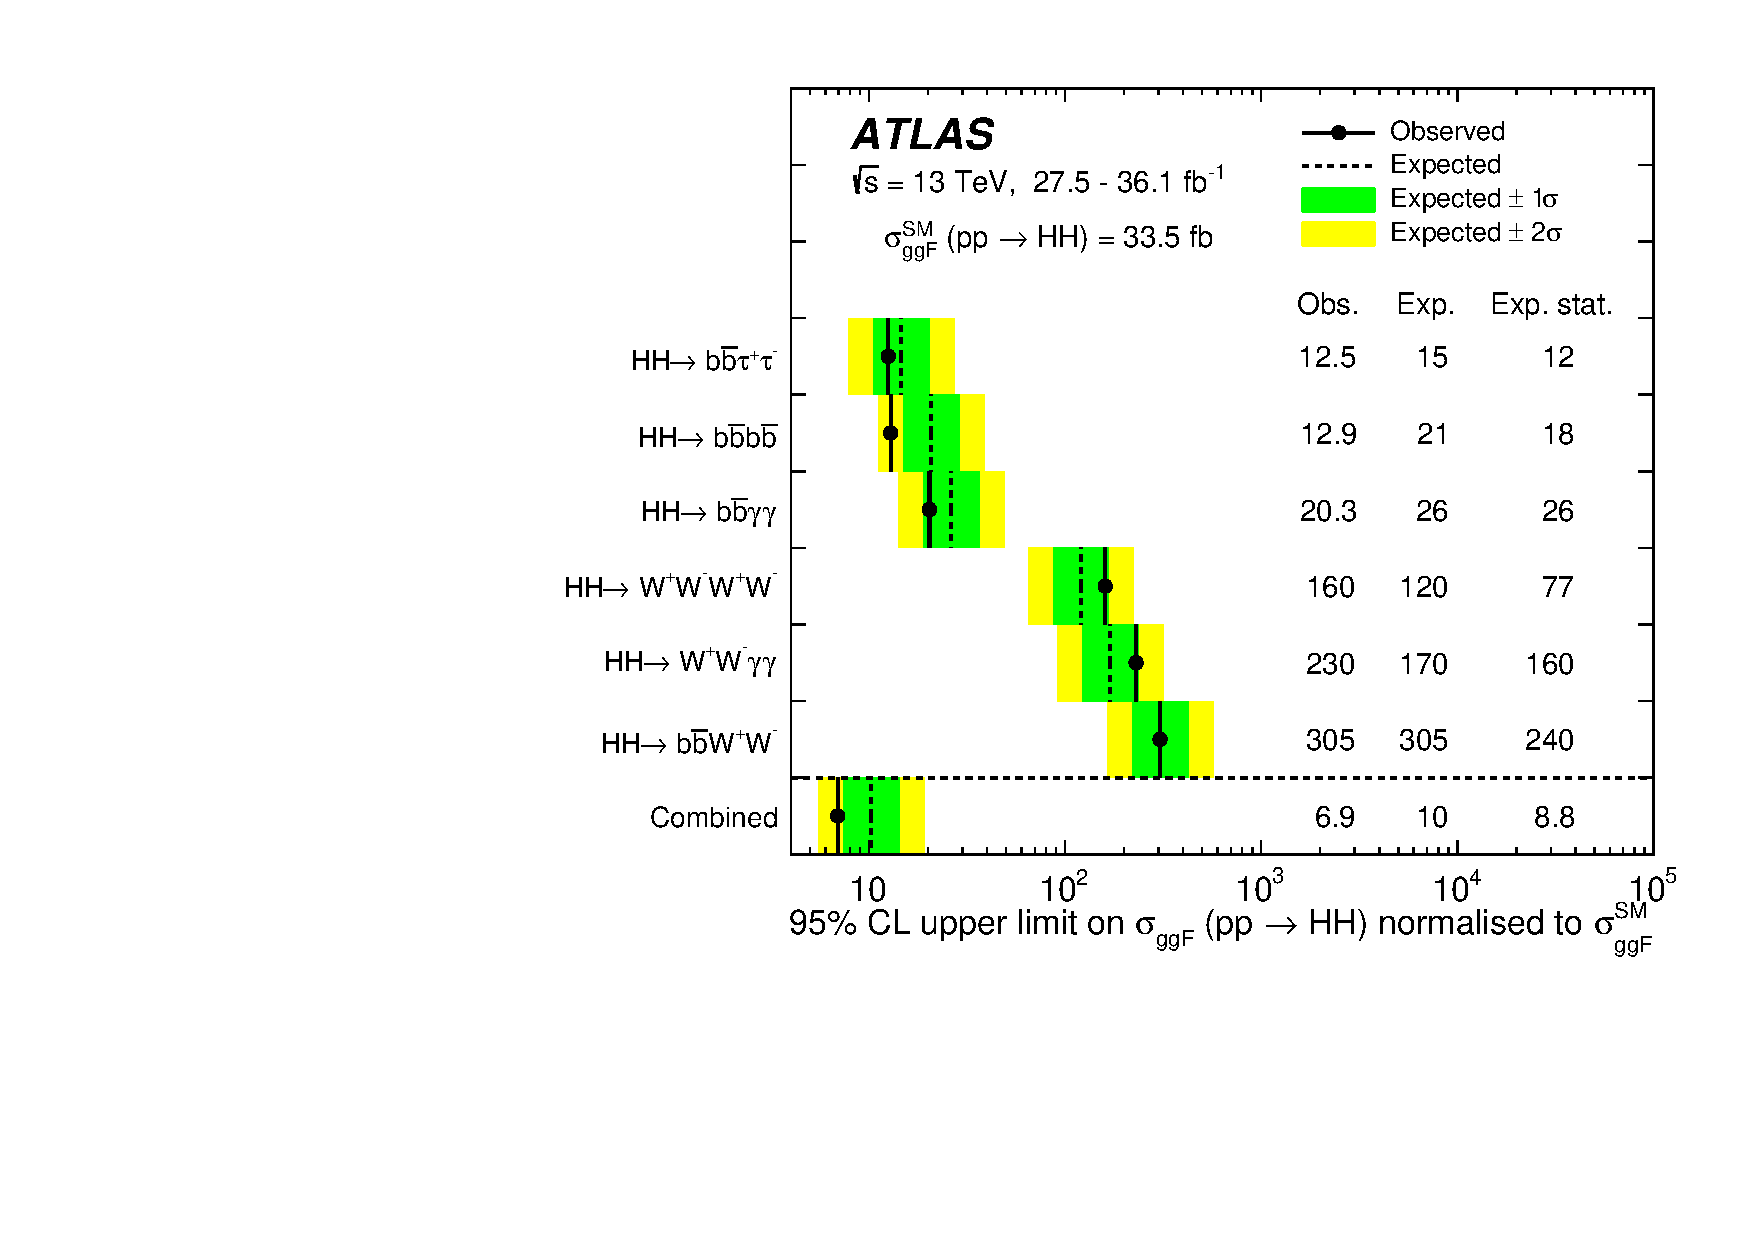
\includegraphics[width=\textwidth]{discussion/results_36ifb}

    \subcaption{Partial Run~2 dataset with an integrated luminosity of \num{27.5} -
      \SI{36.1}{\per\femto\barn}~\cite{HDBS-2018-58}}%
    \label{fig:atlas_run2_36ifb}
  \end{subfigure}\hfill%
  \begin{subfigure}[b]{0.46\textwidth}
    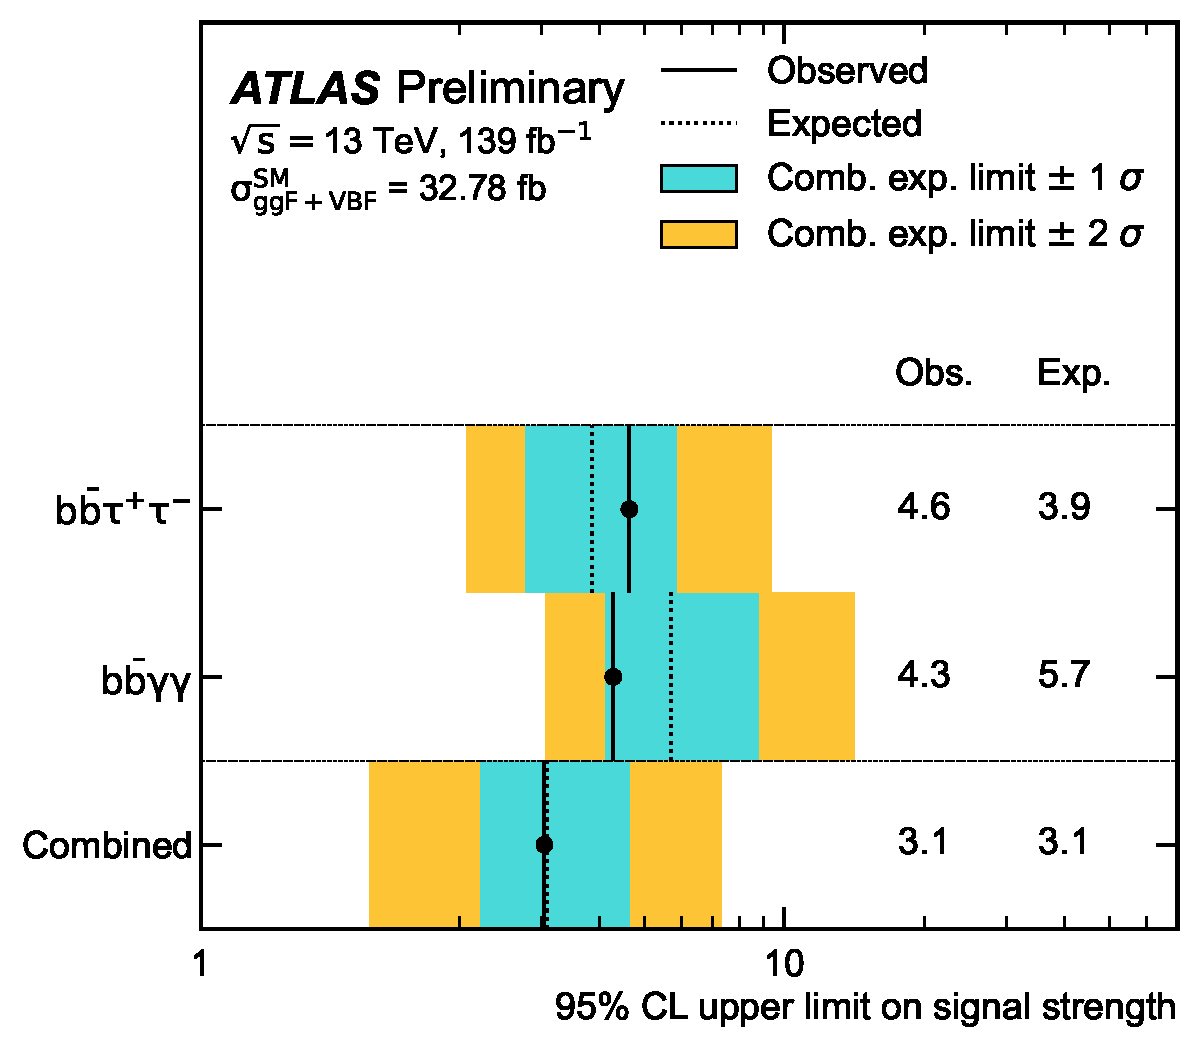
\includegraphics[width=\textwidth]{discussion/results_139ifb}

    \subcaption[margin=5em]{Full Run~2 dataset with an integrated luminosity
      of~\SI{139}{\per\femto\barn}~\cite{ATLAS-CONF-2021-052}}%
    \label{fig:atlas_run2_139ifb}
  \end{subfigure}

  \caption{Comparison of ATLAS results for searches for non-resonant
    SM \HH production from the beginning (a) and end of Run~2 (b) of
    the LHC. Upper limits are shown in terms of the signal strength of
    SM \HH production via \ggF neglecting the VBF production mode in
    (a) and in terms of the combined signal strength of \ggF and VBF
    production mode in (b). Both results are still comparable due to
    the small cross section of VBF \HH production. Addtionally, the
    assumed SM \HH cross sections changed between results due to the
    availability of improved theoretical predictions.  Note the
    different results for bbtautau. }
  \label{fig:atlas_run2_hh_results}
  \todo[inline]{Make my own plot / table for RHS including bbWW and
    possibly 4b? 4b obs.\ 5.4 (exp.\ 8.1)}
\end{figure}

\begin{table}[tbp]
  \centering

  \todo[inline]{Mark preliminary results?}

  \caption{Table of CMS results of searches for non-resonant
    production of Higgs boson pairs with an integrated luminosity of
    \SI{138}{\per\femto\barn}. Upper limits are shown at
    \SI{95}{\percent} CL on the signal strength of the combination of
    the \ggF and VBF production modes.}%
  \label{tab:cms_nonresonant}

  \begin{tabular}{l@{\hskip 2em}SSc}
  \toprule
  \textbf{CMS} (\SI{138}{\per\femto\barn}) & \multicolumn{3}{c}{Upper limit on $\mu_{gg\text{F+VBF}}$ (\SI{95}{\percent} CL)} \\
  \cmidrule{2-4}
  Final state & {Observed} & {Expected} & Reference \\
  \midrule
  $\bbbar\tau^{+}\tau^{-}$ & 3.3 & 5.2 & \cite{CMS-PAS-HIG-20-010} \\
  $\bbbar\gamma\gamma$ & 7.7 & 5.2 & \cite{CMS-HIG-19-018} \\
  $\bbbar\bbbar$ & 3.9 & 7.8 & \cite{CMS-HIG-20-005-PREPRINT} \\
  % Multilepton = ($W^+W^-W^+W^-$, $W^+W^-\tau^+\tau-$, $\tau^+\tau^-\tau^+\tau^-$)
  Multi-lepton  & 21.8 & 19.6 & \cite{CMS-PAS-HIG-21-002} \\
  \bottomrule
\end{tabular}


%%% Local Variables:
%%% mode: latex
%%% TeX-master: "../phd_thesis"
%%% End:

\end{table}

With the currently available dataset and experimental constraints (due
to triggers, reconstruction, identification / isolation) of the ATLAS
experiment for Run~2 of the LHC, the \bbtautau channel achieves a
trade-off between the competing \bbyy and \bbbb channels regarding the
search for SM \HH production. While the \bbyy channel provides access
to events with low \mHH due to the ability to trigger on the signature
of photons with low momentum thresholds (this is particularly
advantageous when considering anomalous values of the Higgs boson
self-couplings, cf.~REFERENCE) and a large background rejection due to
the excellent $\gamma\gamma$ mass resolution, it is subject to the
very small $\PHiggs \to \gamma\gamma$ branching ratio. In contrast,
the largest fraction of SM \HH events are expected in the \bbbb final
state, however, the measurement of SM \HH production in this channel
is challenging due to the fully hadronic final state being subject to
large multi-jet backgrounds and difficulties in selecting signal
candidate events at trigger-level\footnote{There are also
  combinatorial difficulties in reconstructing $\PHiggs \to \bbbar$
  candidates in the \bbbb channel where it can be ambiguous
  (particularly at low \mHH) how $b$-jets are paired into Higgs boson
  candidates. However, SM \HH production is produced at sufficiently
  high \mHH such that this is not really a huge issue.}. The \bbtautau
final state, particulary in the \hadhad channel due to less prevalence
of \ttbar backgrounds compared to the \lephad channel, is very
sensitive to SM \HH production as signal events can be efficiently
selected using \tauhadvis triggers due to their hard \mHH
spectrum. The presence of \tauhadvis (and electrons / muons) provides
large rejection power against multi-jet backgrounds compared to the
\bbbb channel. Moreover, the fraction of SM \HH events decaying into
\bbtautau final states is significantly larger than that of \bbyy.

In~\Cref{fig:atlas_run2_36ifb,fig:atlas_run2_139ifb} a comparison
between searches for SM \HH production using the partial and full
Run~2 $pp$-collision dataset collected with the ATLAS detector is
given. The search for SM \HH production in the \bbtautau final state
using data collected at the beginning of Run~2 of the LHC
(\SI{36.1}{\per\femto\barn}) yielded an expected upper limit on
$\mu_{\ggF}$ of 14.8~\cite{HIGG-2016-16-witherratum}. While upper
limits are set on a different parameter and different theory cross
sections for the signal are assumed, the results can still be compared
to the one obtained using the full Run~2 $pp$-collision dataset
(\SI{139}{\per\femto\barn}) since the change cross section is small
and the contribution of the VBF production mode can be neglected for
the purpose of this comparison. The analysis of the full Run~2
$pp$-collision dataset presented in this work yields an expected upper
limit on $\mu_{\ggF+\text{VBF}}$ of 3.9, far exceeding the expectation
from a naive scaling of the previous result according to the increase
in integrated luminosity which would yield an expected upper limit of
about~7.\footnote{Assuming a purely statistically limited measurement
  that scales with integrated luminosity like a Poisson counting
  experiment. The change in the upper limit depends on the expected
  number of background events and thus cannot be soley described by
  the change in integrated luminosity. Depending on the scenario, the
  extrapolation of the upper limit of \num{14.8} from
  \SI{36.1}{\per\femto\barn} to \SI{139}{\per\femto\barn} ranges
  between \num{6.5} and \num{7.5}.}  This improvement is primarily due
to two reasons:
\begin{itemize}

\item Large improvements in signal sensitivity due to improvements in
  $b$-jet tagging, \tauhadvis reconstruction and identification, which
  allowed to relax identification requirements while maintaining
  background rates comparable to the previous analysis. %
  %                      Old        New
  % LepHad (SLT+LTT)     3.2 %      5.1 %
  % HadHad               1.9 %      4.1 %
  As a result, the signal acceptance improved by a factor of about 2
  (about 1.5) in the \hadhad (\lephad) channel.

\item The increase in integrated luminosity of the collected dataset
  increases the population of signal-like phase spaces allowing for
  better exploitation of the distinct signature of Higgs boson pair
  production.

  This is a side-effect of the constraints imposed on the re-binning
  algorithms applied to the MVA discriminants. The limits on the
  minimum number of background events (expected) and maximum
  statistical uncertainty on the background estimate for a good bin
  introduce a dependency of the re-binning algorithm on the integrated
  luminosity of data and simulation. Thus an increase in integrated
  luminosity allows for narrower bins in the high MVA score region
  improving signal sensitivity. This is not a general feature but due
  to the large discrimination power of the MVA discriminants used to
  extract the SM \HH signal.\todo{It would be good to know how large
    this effect is?}
\end{itemize}

\todo[inline]{Comparison with CMS results. Why is ATLAS better?}

An outlook on the future of non-resonant SM \HH searches with the
ATLAS experiment is provided by an extrapolation of the search
presented in this work to the end of the HL-LHC project with a final
integrated luminosity of \SI{3000}{\per\femto\barn} at a $pp$ center
of mass energy of $\sqrt{s} = \SI{14}{\TeV}$. This extrapolation was
performed by the ATLAS collaboration as part of
Ref.~\cite{ATL-PHYS-PUB-2021-044}.

The analysis is scaled to an integrated luminosity of
\SI{3000}{\per\femto\barn}, accounting for changes in signal and
background cross sections due to the increase in $\sqrt{s}$. Assuming
that the overall performance can be maintained even in the difficult
pile-up conditions of the HL-LHC. Moreover, a baseline scheme
describing the time evolution of systematic uncertainties to Run~4-5
adopted fro the LHC-WG is used~\cite{ATL-PHYS-PUB-2019-006}.

Under these assumptions a discovery significance of $2.8\,\sigma$ for
the measurement in the \bbtautau channel can be achieved for the
non-resonant \HH production in the SM. When combining both the
\bbtautau and \bbyy search channels channels, which is extrapolated to
yield a discovery significance of $2.2$ under similar
assumptions~\cite{ATL-PHYS-PUB-2022-001}, would allow to claim
evidence with a significance of $3.2\,\sigma$ for the
combination~\cite{ATL-PHYS-PUB-2022-005}. A discovery of non-resonant
\HH production in the SM at the end of the HL-LHC would be realistic
provided a combination of the three most sensitive channels
(\bbtautau, \bbyy, \bbbb) between the ATLAS and CMS collaboration can
be performed and the performance of detectors and analyses can be
improved in spite of the more difficult conditions at the HL-LHC.

\todo[inline]{Are there CMS prospect studies?}

\begin{itemize}
\item Expected statistical significance of $2.8\,\sigma$ using
  best-guess assumptions regarding the evolution of systematic
  uncertainties going from Run~2 to Run~4 of the LHC.
\end{itemize}


\subsection{Search for resonant production of Higgs boson pairs}

How does the excess fit into other results?

$4b$: \SI{6.5}{\femto\barn} (exp.\ \SIpmerr{8.15}{+1.17}{-0.77}{\femto\barn})

\todo[inline]{Discussion excess: Modelling of collinear taus?}


%%% Local Variables:
%%% mode: latex
%%% TeX-master: "../../phd_thesis"
%%% End:
